%%
%% sample document for AAMAS'19 conference
%%
%% modified from sample-sigconf.tex
%%
%% see ACM instructions acmguide.pdf
%%
%% AAMAS-specific questions? F.A.Oliehoek@tudelft.nl
%%

\documentclass[sigconf]{aamas}  % do not change this line!

%% your usepackages here, for example:
\usepackage{booktabs}

%% do not change the following lines
\usepackage{flushend}
\setcopyright{ifaamas}  % do not change this line!
\acmDOI{doi}  % do not change this line!
\acmISBN{}  % do not change this line!
\acmConference[AAMAS'20]{Proc.\@ of the 19th International Conference on Autonomous Agents and Multiagent Systems (AAMAS 2020), B.~An, N.~Yorke-Smith, A.~El~Fallah~Seghrouchni, G.~Sukthankar (eds.)}{May 2020}{Auckland, New Zealand}  % do not change this line!
\acmYear{2020}  % do not change this line!
\copyrightyear{2020}  % do not change this line!
\acmPrice{}  % do not change this line!


%% the rest of your preamble here %%check and remove later
\usepackage{amsmath}
\usepackage{amsthm}
\usepackage{algorithm}
\usepackage{algorithmic}
\usepackage{enumitem}
\usepackage{color}
%\newtheorem{theorem}{Theorem} % {\bfseries}{\itshape}
\newtheorem{observation}{Observation} % {\bfseries}{\itshape}
%\newtheorem{lemma}{Lemma}{\bfseries}{\itshape}
\newcommand{\prob}{\textsc{EpiControl}}
\newcommand{\probone}{\textsc{1stage-EpiControl}}
\newcommand{\probtwo}{\textsc{2stage-EpiControl}}
\newcommand{\probdelay}{\textsc{EpiControlDelayInfo}}
\newcommand{\algo}{\textsc{saaRound}}
\newcommand{\algodelay}{\textsc{saaDelayRound}}
\newcommand{\red}[1]{\textcolor{red}{#1}}
\newcommand{\X}{\mathbf{X}}
\newcommand{\B}{\mathcal{B}}
\newcommand{\expinf}{\texttt{eInf}}
\newcommand{\src}{\mathbf{s}}
\newcommand{\ssrc}{\texttt{src}}
\newcommand{\info}{\texttt{info}}

%%%%%%%%%%%%%%%%%%%%%%%%%%%%%%%%%%%%%%%%%%%%%%%%%%%%%%%%%%%%%%%%%%%%%%%%%%%%%%%%%%%%%%%%%%%%%%%%%%%%%%%%%

\begin{document}

\title{Designing Near-Optimal Temporal Interventions to Contain Epidemics}  % put your title here!
%\titlenote{Produces the permission block, and copyright information}

% AAMAS: as appropriate, uncomment one subtitle line; check the CFP
%\subtitle{Extended Abstract}
%\subtitle{Blue Sky Ideas Track}
%\subtitle{JAAMAS Track}
%\subtitle{Demonstration}
%\subtitle{Doctoral Consortium}

% AAMAS: submissions are anonymous for most tracks
\author{Paper \#1460}  % put your paper number here!

%% example of author block for camera ready version of accepted papers: don't use for anonymous submissions
%
%\author{Ben Trovato}
%\authornote{Dr.~Trovato insisted his name be first.}
%\orcid{1234-5678-9012}
%\affiliation{%
%  \institution{Institute for Clarity in Documentation}
%  \streetaddress{P.O. Box 1212}
%  \city{Dublin} 
%  \state{Ohio} 
%  \postcode{43017-6221}
%}
%\email{trovato@corporation.com}
%
%\author{G.K.M. Tobin}
%\authornote{The secretary disavows any knowledge of this author's actions.}
%\affiliation{%
%  \institution{Institute for Clarity in Documentation}
%  \streetaddress{P.O. Box 1212}
%  \city{Dublin} 
%  \state{Ohio} 
%  \postcode{43017-6221}
%}
%\email{webmaster@marysville-ohio.com}
%
%\author{Lars Th{\o}rv{\"a}ld}
%\authornote{This author is the
%  one who did all the really hard work.}
%\affiliation{%
%  \institution{The Th{\o}rv{\"a}ld Group}
%  \streetaddress{1 Th{\o}rv{\"a}ld Circle}
%  \city{Hekla} 
%  \country{Iceland}}
%\email{larst@affiliation.org}
%
%\author{Valerie B\'eranger}
%\affiliation{%
%  \institution{Inria Paris-Rocquencourt}
%  \city{Rocquencourt}
%  \country{France}
%}
%\author{Aparna Patel} 
%\affiliation{%
% \institution{Rajiv Gandhi University}
% \streetaddress{Rono-Hills}
% \city{Doimukh} 
% \state{Arunachal Pradesh}
% \country{India}}
%\author{Huifen Chan}
%\affiliation{%
%  \institution{Tsinghua University}
%  \streetaddress{30 Shuangqing Rd}
%  \city{Haidian Qu} 
%  \state{Beijing Shi}
%  \country{China}
%}
%
%\author{Charles Palmer}
%\affiliation{%
%  \institution{Palmer Research Laboratories}
%  \streetaddress{8600 Datapoint Drive}
%  \city{San Antonio}
%  \state{Texas} 
%  \postcode{78229}}
%\email{cpalmer@prl.com}
%
%\author{John Smith}
%\affiliation{\institution{The Th{\o}rv{\"a}ld Group}}
%\email{jsmith@affiliation.org}
%
%\author{Julius P.~Kumquat}
%\affiliation{\institution{The Kumquat Consortium}}
%\email{jpkumquat@consortium.net}
%
%% The example's default list of authors is too long for headers
%\renewcommand{\shortauthors}{B. Trovato et al.}


\begin{abstract}  % put your abstract here!
Vaccination is a standard public health intervention for controlling the spread of epidemics. However, there is typically limited supply of vaccines, and therefore, their deployment needs to be optimized. Further, vaccines are produced over time, so the strategies have to be temporal. We study the problem \prob{} of designing temporal vaccination strategies, within available budget constraints, to minimize the spread of an outbreak, and with delay in information of the epidemic state.

This is a challenging stochastic optimization problem. 
We design the first algorithm with a rigorous approximation guarantee for this problem.
Our main technique is a combination of linear programming based rounding, along with the 
sample average approximation technique. With additional pruning techniques, we are able to scale
our algorithm to networks with millions of nodes.
We find the approximation factor is significantly better than the worst case bound,
and, in practice, is a small constant factor. Further, our method shows significantly better performance
than all prior heuristics for this problem.
\end{abstract}


\keywords{computational epidemiology; network science; optimization; computational social science}  % put your semicolon-separated keywords here!

\maketitle


\section{Introduction}
\label{sec:intro}

Vaccination and social distancing are the primary strategies for controlling the spread of epidemic outbreaks
\cite{medlock:science09,Ogura2017,halloran:pnas08,lofgren:pnas14,zhang2015controlling,YaoSDM2014,AAAI1816714,PreciadoVM13_2,PreciadoVM13,PreciadoVM14,Aspnes:2005}.
The production of vaccines is expensive and time intensive, and so there is always a shortage of
vaccine supply \cite{cdc:temporal}. As a result, there is a lot of interest in evaluating different kinds of
interventions \cite{halloran:pnas08,lofgren:pnas14}, and finding optimal interventions \cite{medlock:science09}.
The spread of epidemics is very complex, and SIR type diffusion processes (and variations) are commonly used:
Informally, each infected individual $u$ (in state I) spreads the infection to each susceptible neighbor $v$ 
(in state S) with transmission probability $p(u, v)$ (or $p$, if this is uniform for all edges); 
this is defined formally in Section \ref{sec:prelim}.
These can be modeled as system of differential equations \cite{medlock:science09,AAAI1816714,venkataramanan:ichi17}, or as stochastic
agent based models on social contact networks, e.g., \cite{marathe:cacm13}.
Differential equation models are small enough that they can be solved optimally by simple brute-force
local search methods \cite{medlock:science09}.

However, network and agent based models cannot be easily optimized this way. 
In this paper, we study problem \prob{} of \emph{designing temporal vaccination strategies to minimize
the expected outbreak size in an SIR epidemic process on a network $G=(V, E)$}.
There is a lot of relevant prior work on this topic, and can be split along the following lines:
(1) Optimization in the SI/SIS type models, in static ot dynamic networks, e.g.,
\cite{PreciadoVM13_2,PreciadoVM13,PreciadoVM14,SahaSDM15,Ogura2017}. Much of this work is based on
controlling spectral properties, but does not give any guaranteed bounds on the expected outbreak size;
(2) Firefighter problem, which can be viewed as \prob{} on SI model with with $p=1$, e.g.,
\cite{anshelevich09,Finbow2009TheFP}. Rigorous bounds are known for the number infected and saved.
However, this has not been studied much for the case where $p<1$, except \cite{DBLP:journals/corr/abs-1711-08237},
which only gives rigorous algorithms for trees.
A special case of this problem is with work of \cite{Aspnes:2005}, which considers \prob{} but with
the intervention specified at time 0;
(3) Static interventions in SIR models, e.g., \cite{zhang2015controlling,YaoSDM2014}, which also do not
directly bound the expected outbreak size,
(4) Heuristics for picking nodes based on degree or centrality, e.g., \cite{PhysRevLett.91.247901,Miller2007EffectiveVS},
which work for all models but give no guarantees.
In summary, none of the prior results give rigorous results for \prob{}, to minimize the expected
number of infections, with budget constraints over time, in SIR models of epidemics, with transmission probability less than $1$.

\noindent
\textbf{Our results.}
\emph{We present the first approximation algorithm for \prob{} with rigorous guarantees.}
Our specific contributions are described below.
\begin{itemize}
\item
We design algorithm \algo{} for selecting the sets of nodes to vaccinate at different times,
within a given set of temporal budget constraints. We show a rigorous worst case approximation guarantee on
the performance of \algo{}, which is logarithmic in the number of paths in sampled subgraphs of $G$;
this is typically significantly smaller than the number of paths in $G$, so that
in practice, \algo{} has a much smaller approximation ratio.
Our main technical ideas are rounding a linear programming (LP) relaxation, along with the sample average technique.
\item
We augment \algo{} with a sparsification step, which significantly reduces the size of the LP, and
is able to scale to networks with millions of nodes and edges.
\item 
We evaluate our algorithms on diverse real and random networks.
We show that \algo{} has an approximation ratio very close to $1$, significantly better than the worst case guarantee we prove rigorously. 
We find that \algo{} outperforms two of the most commonly used baselines for intervention design.
We also examine the structure of solutions, and find significant differences in the characteristics of nodes
picked in different stages.
\end{itemize}

\noindent
\textbf{Public health impact.}
At the start of every flu outbreak, and during major pandemics, there is a lot of interest from the CDC and other public health agencies on finding optimal solutions in different models, e.g., \cite{medlock:science09,halloran:pnas08,lofgren:pnas14,venkataramanan:ichi17}. These can be used to guide policies when there are shortages, including the logistics of where vaccines should be deployed \cite{venkataramanan:ichi17}. Our methods help designing near-optimal policies using agent based models, which have been found to be more useful in planning for large outbreaks, e.g., \cite{halloran:pnas08,lofgren:pnas14,eubank:nature04,gk06}.

%%%In most diseases, e.g. flu, the final policies have to be \emph{implementable}. This is ill-defined, but one characteristic is that the interventions should not target specific individuals, but could be defined by broader categories, e.g., age (as in the CDC guidelines). In such a case, the solution from a method like ours will not translate into an implementable policy. However, our algorithms can be used for a group level intervention design problem, as in \cite{zhang2015controlling}, which would give more implementable solutions.


\section{Notation and problems}
\label{sec:prelim}

\noindent
\textbf{Network and disease model} (summarized in Table \ref{tab:notation}).
Let $G = (V, E)$ be a contact graph where $V$ is the set of people (or nodes) and $e = (u, v) \in E$ if nodes $u, v \in V$ come into direct contact, which can allow a disease to spread. Let $n = |V|$ be the number of nodes in graph $G$. 
We assume a simple SIR model of disease spread \cite{marathe:cacm13}, in which each node is in one of the following states:
susceptible (S), infectious (I) or recovered (R).
The epidemic starts at one or more externally infected nodes, and spreads from an infected node $u$ to each susceptible
neighbor $v$ with probability $p$. An infected node becomes recovered in the next time step.
We assume $s_v$ is the probability that $v$ is initially infected; $\mathbf{s}$ denotes the initial infection vector.
As is typical in public health analyses, we will assume a small number of random initial infections.\\
\textbf{Note.} The SIR model generalizes the well studied \emph{independent cascades} model \cite{kempe:kdd03}.
Also, there are lots of variations of the SIR model, such as:
varying transmission probability $p(u, v)$ on each edge $(u, v)$,
with an exposed state, varying infectious duration, etc.;
most of our results extend to the general models.

\begin{figure}
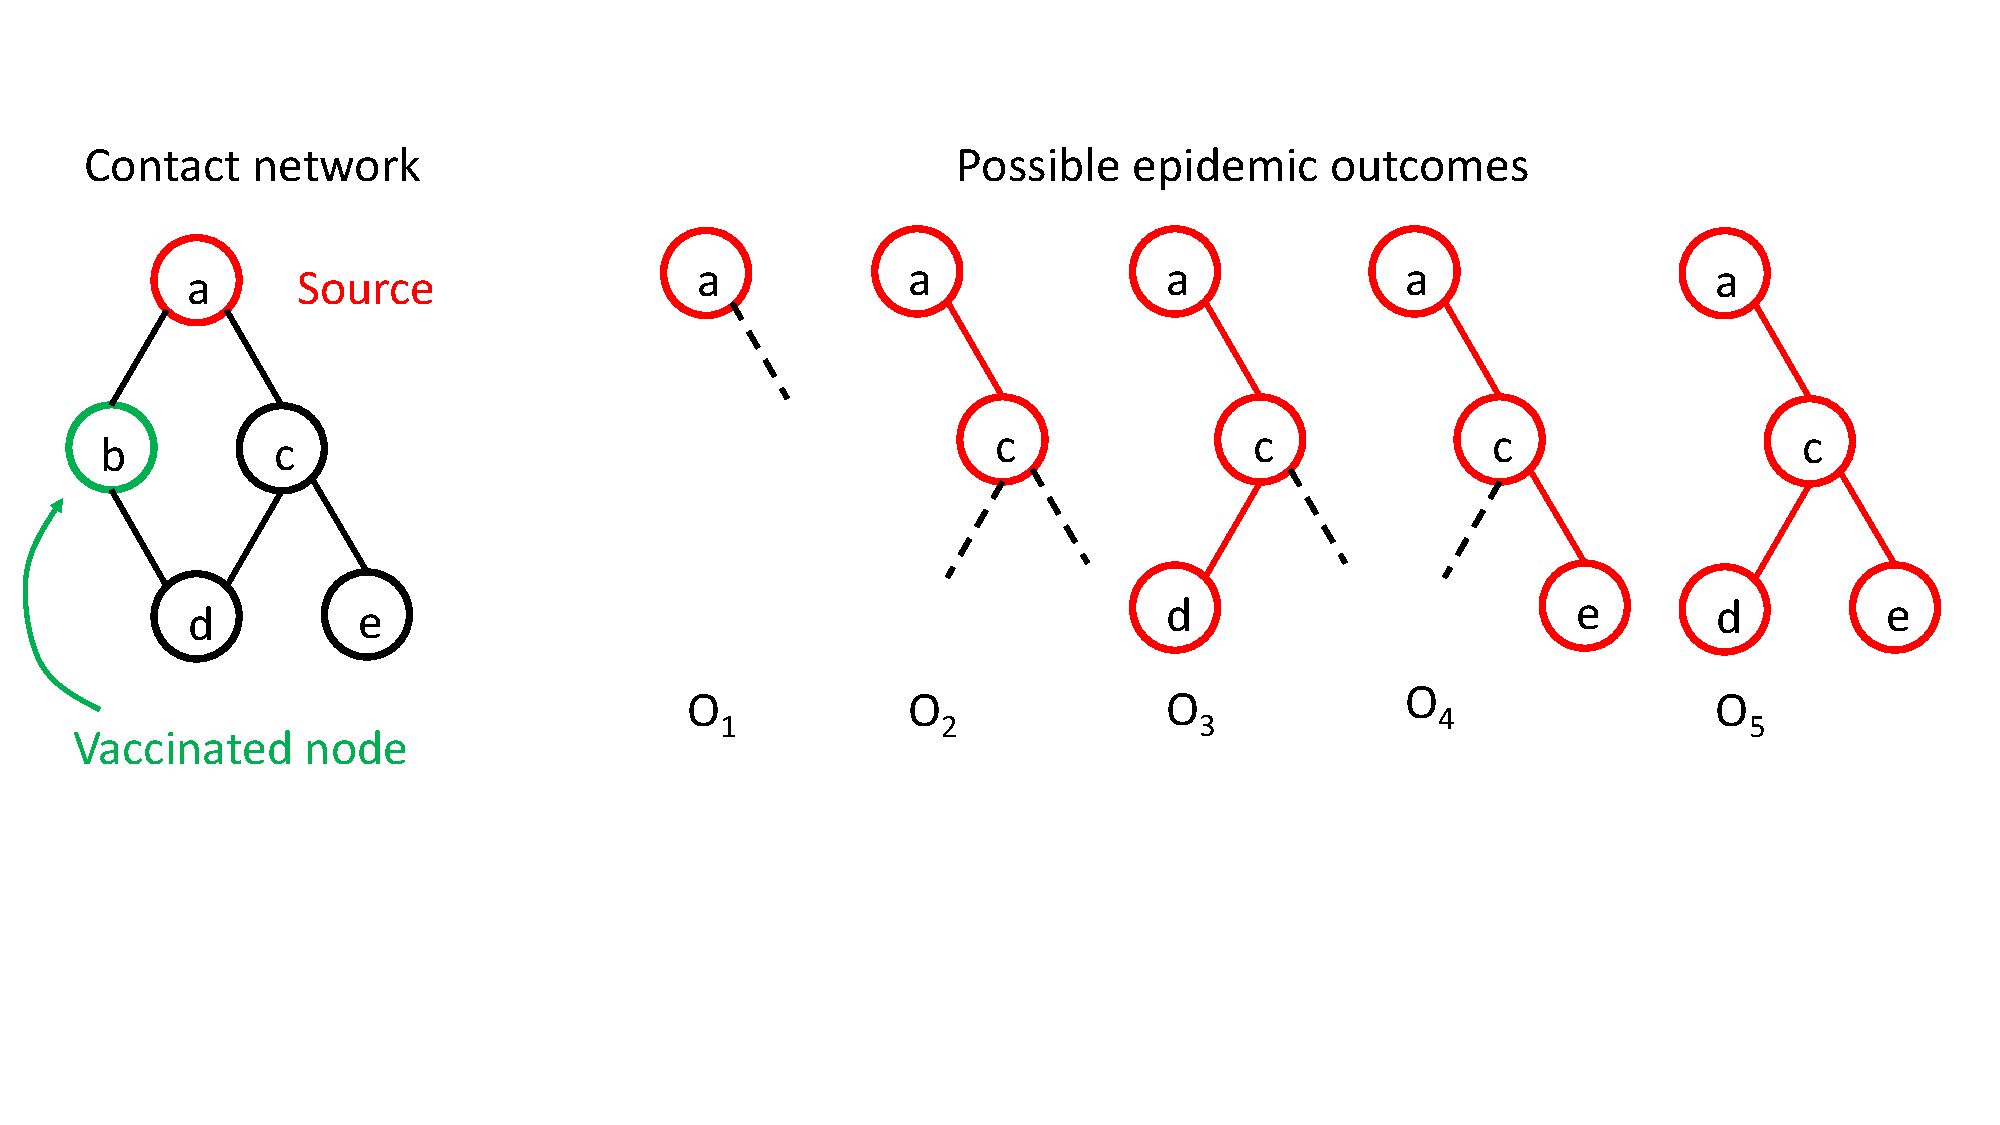
\includegraphics[scale=0.25]{figures/example.pdf}
\caption{Example illustrating the SIR model: the contact network $G=(V, E)$ is shown in the left,
with $V=\{a, b, c, d, e\}$ (shown in circles), and edges as solid lines.
Node $a$ is initially infected, and node $b$ is vaccinated. The five subgraphs $O_1, O_2, O_3, O_4, O_5$
(on the right) are possible stochastic outcomes in the SIR model.}
\label{fig:example}
\end{figure}

\noindent
\textbf{Interventions and objective.}
We use $x_{vt}$ as an indicator variable, which is $1$ if node $v$ gets vaccinated at time $t$.
Let $\X_t=\{v: x_{vt}=1, v\in V\}$ denote the set of nodes vaccinated at time $t$, and 
$\X=\{\X_t: t\in\mathcal{T}\}$ denote the combined set of all temporal vaccination
decisions; here $\mathcal{T}=\{t_0, t_1,\ldots\}$ denotes a set of times at which decisions are to be made.
We assume the vaccine is immediately effective; our methods can be extended to handle limited efficacy vaccines.
We assume a budget vector $\B=(B_t: t\in\mathcal{T})$, which specifies the number of vaccines available
at each time $t\in\mathcal{T}$. We focus on the following objective:
$\expinf(G, \src, \mathcal{T}, \X)$, which denotes the expected number of infections that occur if the epidemic
starts with the vector $\src$, and nodes are vaccinated at each time $t\in\mathcal{T}$, as per the vector $\X_t$.
We use simpler notation to denote the expected number of infections in the following special cases:\\
(1) No vaccination case: $\expinf(G, \src)$, when no vaccinations are done,\\
(2) Single stage: $\expinf(G, \src, \X_0)$, when vaccinations are only done at time 0 for nodes in set $\X_0$, and\\
(3) Two stage: $\expinf(G, \src, \X_0, \X_T)$, when vaccinations are done at two time steps,
namely $0$ and $T$.\\
(4) We drop $G$ and $\src$, when it is clear from the context.

\begin{table}[!h]
\centering
\begin{footnotesize}
\begin{tabular}{|l|l|}
\hline
\textbf{Notation} & \textbf{Definition}\\
$G=(V, E)$ & Graph\\
$\src$ & Source distribution\\
$p$, $p(u, v)$ & Transmission probability\\
$x_{vt}$ & Indicator for node $v$ vaccinated at time $t$\\
$\X_t$ & Set of nodes vaccinated at time $t$\\
$\X$ & Set of all $\X_t$'s\\
$\mathcal{T}$ & Time steps at which intervention is done\\
$\expinf(G, \src, \mathcal{T}, \X)$ & Expected number of infections with intervention $\X$\\
$\expinf(G, \src, \X_0)$ & Exp. \#infections for single stage with intervention $\X_0$\\
$\expinf(G, \src, \X_0, \X_T)$ & Exp. \#infections for two stage version\\
\prob & Designing temporal intervention to minimize $\expinf$\\
\probone & Problem with one stage\\
\probtwo & Problem with two stage\\
$(\alpha, \beta)$ approximation & Bicriteria approximation factor\\
\hline
\end{tabular}
\end{footnotesize}
\caption{Summary of notation used in the paper.}
\label{tab:notation}
\end{table}

\noindent
\textbf{Example.} Figure \ref{fig:example} shows the SIR model and the definitions of the above quantities
on a graph $G$ with five nodes. Initially, node $a$ is infected, and $b$ is vaccinated. 
In the SIR model, the disease spreads from an infected node to each susceptible neighbor with probability $p$,
and does not spread with probability $1-p$. Therefore, we have five possible stochastic outcomes $O_1,\ldots,O_5$,
which occur with probabilities $1-p$, $p(1-p)^2$, $p^2(1-p)$, $p^2(1-p)$, and $p^3$, respectively.
Suppose we have $\mathcal{T}=\{0\}$. Then, $x_{b0}=1$, and $\X=\X_0=\{b\}$.
We have 
\[
\expinf(\X)= (1-p) +2p(1-p)^2+2\cdot 3 p^2(1-p) + 4p^3
\]

\noindent
\textbf{The temporal vaccination problem (\prob).}\\
\underline{Given}: contact network $G=(V, E)$, initial infection vector $\mathbf{s}$, set of times $\mathcal{T}$,
budget vector $(B_t: t\in\mathcal{T})$\\
\underline{Compute}: a set $\X$ of intervention sets at each time, 
such that $\expinf(G, \src, \mathcal{T}, \X)$ is minimized, and $\sum_v x_{vt} \leq B_t$ for all $t\in\mathcal{T}$.

\noindent
\textbf{Special cases of the \prob{} problem.}
\begin{itemize}
\item
\textbf{Single stage vaccination problem (\probone):} given budget $B_0$, choose $\X_0$ such that $|\X_0|\leq B_0$
and $\expinf(G, \src, \X_0)$ is minimized.
\item
\textbf{Two stage vaccination problem (\probtwo):} given budget $B_0, B_T$, choose $\X_0, \X_T$ such that
$|\X_0|\leq B_0$, $|\X_T|\leq B_T$, and $\expinf(G, \src, \X_0, \X_T)$ is minimized.
\end{itemize}

\noindent
\textbf{Bi-criteria approximate solution.}
We say that an intervention $\X=\{\X_t: t\in\mathcal{T}\}$ is an $(\alpha, \beta)$-approximation if:
(1) $|X_t|\leq \alpha B_t$, for each $t$, and
(2) $\expinf(G, \src, \mathcal{T}, \X)\leq \beta \expinf(G, \src, \mathcal{T}, \X^*)$, where
$\X^*$ is an optimal solution to the instance of \prob{}.
We say an algorithm is an $(\alpha, \beta)$-approximation algorithm, if it gives solutions with this factor.



\section{Our approach}
\label{sec:method}

Our algorithm \algo{} uses a linear programming rounding technique, combined with the sample average approximation
technique from stochastic optimization. We then show that this can be significantly speeded up by a more compact LP.

\subsection{Algorithm \algo{}}

%%We start with some definitions needed for the algorithm. Let $H_j=(V, E_j)$ denote a random subgraph of $G$,
%%where each edge $e\in E$ is selected to be in $E_j$ with probability $p$. 
%%Let $\src^{(j)}$ denote the set of source nodes in $H_j$, and
%%let $\mathcal{P}_{vj}$ be the set of paths from sources to $v$ in $H_j$. 
%%Let $N_{vj} = |\mathcal{P}_{vj}|$ be the number of paths from any source to $v$ in $H_j$. 
%%Let $N = max_{(v,j)}  N_{vj}$ be the maximum number of paths from sources to a node in any of the sampled
%%graphs. Let $y_{vj}$ denote the indicator variable to check whether node $v$ is reachable from any source in $H_j$.
%%As defined earlier, $x_{vt}$ is the indicator that node $v$ is vaccinated at time $t$.


\begin{algorithm}{}
\small
\caption{\small $\algo{}$\\
\textbf{Input:} $G, \src, \mathcal{T}, B_t$ for $t\in\mathcal{T}$\\
\textbf{Output:} $\X=\{\X_t: t\in\mathcal{T}\}$
}
\label{alg:saaround}
\begin{algorithmic}[1]
\STATE
Construct a sampled graph $H_j=(V, E_j)$, for $j=1,\ldots,H_M$, by picking each edge $e\in E$ to be in $E_j$
with probability $p$. Also pick a set of sources $\ssrc(H_j)$ by sampling from $\src$
\STATE
Run breadth first search (BFS) in each $H_j$ from the nodes in $\ssrc(H_j)$.
Let $V_{j,t}$ denote the set of all nodes at level $t$ in the BFS tree in $H_j$ 
(with the nodes in $\ssrc(H_j)$ at level $0$); let $V_{j,\geq t}=\cup_{t'\geq t} V_{j,t}$ denote
the set of all nodes at level $t$ or more.
\STATE
Solve the following linear program ($LP_{saa}$)
\begin{eqnarray}
\label{eqn:obj}
(LP_{saa}) \qquad  \min \frac{1}{M}\sum_j \sum_v y_{vj} && \\
\label{eqn:xy}
\forall u \in V_{j, \geq t} - \ssrc(H_j), \forall t:\ y_{uj} &\leq& 1 - x_{ut} \\
\label{eqn:xy2}
\forall u \in \ssrc(H_j), \forall t:\ y_{uj} &\leq& 1 - x_{u0} \\
\label{eqn1}
\forall j, \forall u\in V, \; (w, u)\in E_j:\ y_{uj} &\geq& y_{wj} - \sum_{t: u \in V_{j, \geq t}} x_{ut}\\
\label{eqn:src}
\forall j, \forall s \in src(H_j):\ y_{sj} &=& 1\\
\label{eqn:budget}
\forall t\in\mathcal{T}:\ \sum_u x_{ut} &\leq& B_t\\
%\label{eqn:uniqt}
%\forall u,\ \sum_t x_{ut} &\leq& 1\\
\label{eqn:01}
\mbox{All variables} &\in& [0, 1]
\end{eqnarray}
\STATE
Let $x, y$ be the optimal fractional solution to (LP).
We round it to an integral solution in the following manner
\begin{enumerate}
\item
Round $Y_{vj} = 1$ for each $(v,j)$ if $y_{vj} \geq \frac{1}{2}$, otherwise set $Y_{vj} = 0$.
\item
For each $v, t$, set $X_{vt}=1$ with probability $\min\{1, 2 x_{vt}\log(4nMN)\}$. 
\item
$X_t=\{v: X_{vt}=1\}$ is the set of nodes vaccinated at time $t$, and $X=\cup_t X_t$
is the total set of vaccinated nodes.
\end{enumerate}
\STATE \textbf{return} $X$
\end{algorithmic}
\end{algorithm}

\noindent
\textbf{Intuition behind \algo{} and its analysis.}
Our algorithm involves four key ideas, which are described below, along with an intuitive description of
the steps of the algorithm.
\begin{itemize}[leftmargin=0.1in, noitemsep, topsep=0pt]
\item
Sample average approximation technique: 
The first idea is that it suffices to get a solution which minimizes the average number of
infections in a set of $M$ sampled outcomes, in order to minimize $\expinf(\cdot)$, which is an expectation
over all possible outcomes; we show that it suffices to $M$ is bounded by a polynomial in $n$.
Further, instead of actually using simulation outcomes, Steps 1 and 2 exploit an equivalence between an
SIR process and percolation, making this much more efficient.
\item
Compact integer program:
The problem is challenging even if we have to minimize the average number of infections restricted to
$H_1,\ldots,H_M$. We start with an integer program (IP) which expresses the following constraints: if a node $u$ is not infected in $H_j$
(which is indicated by $y_{uj}=0$), then for every path $P$ from a node in $\ssrc(H_j)$ to $u$ in $H_j$, there must be
a node $v$ which has been vaccinated. Further, node $v$ must have been vaccinated at a time $t< length(P)$, otherwise the
vaccination would not be effective. 
However, such an integer program would have exponentially many constraints (one for each path).
Instead, we design a more compact program,
simply based on states of nodes on an edge, as expressed in constraints (\ref{eqn1}).
This IP is an  integral version of $LP_{saa}$, with the variables required to be binary
which we prove is equivalent.
\item
Linear relaxation:
IP cannot be solved in polynomial time, and we consider a linear relaxation of it, by replacing the binary constraints
by (\ref{eqn01}). The resulting program $LP_{saa}$ involves minimizing a linear objective over a convex polytope,
and so step 3 of \algo{} can be done efficiently to compute the fractional solutions $x, y$.
Also note that since $LP_{saa}$ is optimizing over a larger space (specifically, the convex hull of all the
feasible integral solutions), the objective value in (\ref{eqn:obj}) might be smaller than the integral objective value.
\item
Rounding to an integral solution:
The solution $x$ is fractional, which poses a problem:
if we have $x_{ut}\in(0, 1)$, e.g., a fractional value of $0.2$, it is not clear how to construct
a valid integral solution. In Step 4(1) of \algo{}, we pick all the nodes with $y_{uj}\leq 1/2$ (denoted by $Y_{uj}=0$),
and pick a set of nodes to vaccinate (Step 4(2)), such that every node $u$ with $Y_{uj}=0$ gets disconnected from $\ssrc(H_j)$.
Step 4(2) achieves this by rounding the fractional solution $x$, after appropriate scaling.
This randomized rounding step ensures that the budgets are not violated by much.
This also implies that any node $u$ which gets infected in $H_j$ has $y_{uj}>1/2$, so that the average number
of infections can be bounded by at most twice the fractional objective value.
\end{itemize}

We first start by showing that $LP_{saa}$ is indeed valid, which is not apparent from its structure

\begin{lemma}
The constraints of $LP_{saa}$ are valid.
\end{lemma}
\begin{proof} (Sketch)
Our proof involves showing that the constraints (\ref{eqn:xy}), (\ref{eqn:xy2}), (\ref{eqn1}),
(\ref{eqn:src}), and (\ref{eqn:budget}) are valid, i.e., they are satisfied by an optimal solution.
Consider an optimal solution $\X^*=\{\X^*_t, t\in\mathcal{T}\}$ for the set of sampled graphs
$H_1,\ldots,H_M$. It will follow from Lemma \ref{lemma:conc} later that $\X^*$ is also ``close to''
We define $x^*_{ut}=1$ if $u\in\X^*_t$.
\end{proof}

\begin{lemma}
\label{lem:disconnect}
For any $H_j$, and any node $v\in V$ with $y_{vj} < \frac{1}{2}$, we have
\[
\Pr[\mbox{$v$ is reachable from $\ssrc(H_j)$ in $H_j[V-\X]$}] < \frac{1}{4nM}
\]
where $H_j[V-\X]$ is the graph induced by removing the nodes in $\X$ from $H_j$.
\end{lemma}
\begin{proof}
Let $\mathcal{P}_{vj} = \{P_1, \ldots,P_L\}$ be the  set of paths to node $(v,j)$. 
For a path $P$, let $S(P)=\{(u, t): u\in P\cap V_{it}\}$.
If there exists $(u, t)\in S(P)$ with $2 x_{vt} \log(4nMN) \geq 1$, the rounding ensures that $X_{ut}=1$;
therefore, we only consider the case $2 x_{vt} \log(4nMN)\leq 1$.
Our rounding ensures that we have $\Pr[X_{ut}=1] \geq 2 x_{vt} \log(4nMN)$, so that
$\Pr[\sum_{u, t: u\in P\cap V_{it}} X_{ut} = 0]$ is upper bounded by
$\prod_{(u,t) \in S(P)} \big(1- 2 x_{ut} \log(4nMN)\big) \leq e^{-\sum_{(u, t)\in S(P)} 2 x_{ut} \log(4nMN)}
\leq e^{-\log(4nMN)}= \frac{1}{4nMN}$,
since $\sum_{(u, t)\in S(P)} x_{ut} \geq 1-y_{vj} \geq 1/2$.
Equivalently, the probability that no node from $S(P)$ is picked from $P$ is at most $\frac{1}{4nMN}$;
here we say a node is picked from $S(P)$ if $X_{u,t}=1$ for some $(u, t)\in S(P)$.
By a union bound, the probability that there exists a path $P_i$ such that no node from
$S(P_i)$ is picked is at most $\frac{L}{4nMN}\leq \frac{1}{4nM}$.
Finally, $v$ is reachable from $\ssrc(H_j)$ in $H_j[V-\X]$ if and only if there exists a path $P_i$ such that no node from
$S(P_i)$ is picked, and so the lemma follows.
\end{proof}

Next, we bound the violation in the budget constraints. We use the following Chernoff tail bound.

\begin{theorem} (Theorem 1.1 of \cite{books/daglib/0025902}
Let $Z=\sum_{i=1}^n Z_i$, where $Z_i$ are independently distributed random variables in $[0, 1]$. Then, for any $\epsilon\in(0, 1)$, we have
$\Pr[Z\not\in[(1-\epsilon)E[Z], (1+\epsilon)E[Z]]]\leq 2 exp(-\epsilon^2 E[Z]/3)$


\end{theorem}

\noindent
\begin{lemma}
\label{lem:budget}
With probability at least $1-1/n$, for each $t\in \mathcal{T}$, we have
$|X_t|\leq 4\log(4nMN)B_t$.
\end{lemma}
\begin{proof}
We have $E[\sum_u X_{ut}]\leq \sum_u 2x_{ut}\log(4nMN) \leq 2\log(4nMN)B_t$.
The $X_{ut}$'s are all rounded independently, and so we can apply the Chernoff bound on the sum, which gives
$\Pr[\sum_u X_{ut} > 4\log(4nMN)B_t] \leq exp(-2\log(4nMN)B_t) \leq exp(-2\log(4nMN))= \frac{1}{(4nMN)^2}\leq \frac{1}{16n^2}$.
The number of possible time steps in $\mathcal{T}$ is at most $n$, which implies that the probability that there exists 
$t\in\mathcal{T}$ such that $\sum_u X_{ut} > 4\log(4nMN)B_t$ is at most $n\frac{1}{16n^2}=\frac{1}{16n}\leq 1/n$.
\end{proof}

For a vaccination set $U$, let $Z_j(U)$ be the number of nodes in 
$H_j-U$, which are still reachable from $\ssrc(H_j)$;
note that this includes the sources themselves.
Let $Z(U)=\frac{1}{M}\sum_j Z_j(U)$, and let $\hat{X}_{opt}=\mbox{argmin}_{X'}Z(X')$ be the solution that
achieves the minimum average number of infections in the samples.
Finally, let $X_{opt}=\mbox{argmin}_{X'}\expinf(X')$ be the optimal solution to the $\prob{}$ instance,

\begin{lemma}
\label{lemma:conc}
Let $Z(\cdot)$ be as defined above. If $M\geq 48n\log{n}$, with probability at least $1-1/n$, for every intervention set $U$,
we have $Z(U)\in [\frac{1}{2}\expinf(U), \frac{3}{2}\expinf(U)]$.
\end{lemma}
\begin{proof}
By definition, $Z(U)=\frac{1}{M}\sum_j Z_j(U)$.
We have $E[Z(U)] = E[Z_j(U)]=\expinf(U)$ for all $j$.
By the Chernoff bound, we have
\[
\Pr[MZ(U)\not\in [\frac{1}{2}, \frac{3}{2}]M\expinf(U)]\leq 2exp(-\frac{M}{24}\expinf(U))
\]
We have $\expinf(U)\geq 1$, since there is always at least one infection.
For $M=48n\log{n}$, this probability is at most $2e^{-2n\log{n}} = \frac{2}{e^2e^nn}$.
The number of possible intervention sets is the number of possible sets $U_t\subseteq V$, $t\in\mathcal{T}$,
which is at most $n2^n$.
Therefore, the probability that there exists an intervention set $U$ for which
$Z(U)\not\in [\frac{1}{2}, \frac{3}{2}]\expinf(U)$ is at most $n2^n\cdot \frac{2}{e^2e^nn}\leq \frac{1}{n}$.
\end{proof}

\begin{theorem}
\label{theorem:algo}
Let $X$ denote the vaccination set computed by algorithm \algo{}.
Then, with probability at least $1/2$, we have
$\expinf(X)\leq 6\expinf(X_{opt})$, and for all $t\in\mathcal{T}$, we have
$|X_t|\leq 4\log(4nMN)B_t$.
\end{theorem}
\begin{proof}
Let $\hat{X}_{opt}$ be as defined above. 
By Lemma \ref{lem:disconnect}, for any $v, j$, if $y_{vj} \leq 1/2$, the probability that node $v$ is
reachable from $\ssrc(H_j)$ is at most $\frac{1}{4nM}$.
By a union bound, the probability this does not hold for any $v$ (for a fixed $j$) is at most $\frac{1}{4M}$.
This implies that with probability at least $1-\frac{1}{4nM}$, 
\[
Z_j(X)\leq |\{v: y_{vj}\geq 1/2\}|\leq \sum_{v: y_{vj}\geq 1/2} 2y_{vj} \leq \sum_v 2y_{vj}
\]
By a union bound, with probability at least $1-\frac{M}{4M}=1-\frac{1}{4}$,
we have $Z_j(X)\leq 2\sum_v y_{vj}$, for all $j$.
By definition of $\hat{X}_{opt}$, we have $\frac{1}{M}\sum_j Z_j(X)\leq \frac{1}{M}\sum_{v,j} 2y_{vj} \leq 2Z(\hat{X}_{opt})$,
since the LP solution is also a lower bound on $Z(\hat{X}_{opt})$.
By Lemma \ref{lem:budget}, and a union bound, the condition $|X_t|\leq 4\log(4nMN)B_t$ holds for all $t$,
in addition to $Z(X)\leq 2Z(\hat{X}_{opt})\leq 2Z(X_{opt})$, with probability at least $1-\frac{1}{4}-\frac{1}{n}$,
since $Z(\hat{X}_{opt})\leq Z(X_{opt})$, by definition of $\hat{X}_{opt}$.

By Lemma \ref{lemma:conc}, with probability at least $1-\frac{1}{n}$,
we have $Z(X_{opt})\leq \frac{3}{2}\expinf(X_{opt})$, and
$\frac{1}{2}\expinf(X)\leq Z(X)$. This gives us
\[
\expinf(X)\leq 2Z(X)\leq 4Z(X_{opt})\leq 6\expinf(X_{opt})
\]
Therefore, all the conditions of the theorem hold with probability $\geq 1-\frac{1}{4}-\frac{2}{n}\geq \frac{1}{2}$.
\end{proof}


\subsection{Speeding up \algo{}}

The main bottleneck in \algo{} is the solution of the LP. Pruning methods

\section{Experiments}
\label{sec:experiments}

We study the following questions:
\begin{itemize}
\item
\textbf{Scaling}: how well does \algo{} scale to large networks? How effective are the techniques for choosing the
number of samples and pruning?
\item
\textbf{Approximation Guarantees}: what is the approximation factor of \algo{} in practice? How does it compare with 
the current best methods for intervention design in networks?
\item
\textbf{Effect of multiple stages}: how does the effectiveness of the solution vary with the number of stages
and the budget in each?
\item
\textbf{Characteristics of the solutions}: what kinds of nodes are picked in the solutions at each stage?
\end{itemize}

\subsection{Dataset and Methods}

\noindent
\textbf{Datasets.}
We experiment with three different classes of networks (total of six),
in order to fully explore the effect of network structure on the the results. 
We consider two random networks, namely the small world 
\cite{Kleinberg00thesmall-world}, and the preferential attachment \cite{Barabasi509} models. The parameters used in generation of the random networks is presented in the full version. \cite{sambaturu:AAAI20}. We study the results on the CA-GrQc collaboration network \cite{Leskovec:2007:GED:1217299.1217301}, since it is a type of social network. We also consider synthetic agent based populations for Montgomery County, VA, and Portland, OR, constructed by a first principles approach by \cite{barrett:wsc09,eubank:nature04}. This has been used in several public health studies, e.g., \cite{singh:bmc19}. This network has a rich set of demographic attributes for each node, e.g., age, gender, and income.
The datasets are summarized in Table \ref{tab:datasets}.

\noindent
\textbf{Choosing parameters.}
There is a large space of model parameters over which the analysis could be done. Due to the space limits, and
in order to get the most insights, we choose a subset as descirbed here.
We choose the source distribution $\src$ so that about 10 initial infections are picked.
Following standard practice in public health, e.g., \cite{halloran:pnas08},
we choose three values for the transmission probability $p$ based on the expected number of infections (referred to as the ``attack rate'') 
that result when there are no interventions: we choose a probability $p_{low}$ if the attack rate is $<10\%$ (low),
$p_{med}$ if the attack rate is in $[10\%, 20\%]$ (medium), and
$p_{high}$ if the attack rate is $> 20\%$.
The specific probability values depend on the datasets.
The full version of the paper \cite{sambaturu:AAAI20} shows how the attack rate varies with the probability, and the specific probability values which were chosen.

\begin{table}[!h]
\centering
\begin{tabular}{llll}
\hline
 \textbf{Dataset} & \textbf{Nodes} & \textbf{Edges}   \\ \hline
 Montgomery & 70729 & 198138 \\
 Portland & 1409197 & 8307767 \\
 CA-GrQc & 5242 & 14496\\
 Small World (SW) & 2500 & 14833 \\   
 Preferential1 (PA1) & 1000 & 1996 \\ 
Preferential2 (PA2) & 100000 & 199996 \\ \hline
\end{tabular}
\caption{Description of datasets}
\label{tab:datasets}
\end{table}

\noindent
\textbf{Methods.}
We only focus on one stage (\probone) or two stage (\probtwo) versions of \prob{} here, and use \algo{} to find 
interventions. We use the Gurobi solver \cite{gurobi} to implement \algo{}.
For \probone{}, we consider the following baselines, which select $B$ nodes based on two criteria:
\begin{itemize}
\item
Nodes with the highest degree, which has been a popular approach in a number of papers
\cite{salathe:plos12, Barabasi509}
\item
Nodes with the highest eigenscore: this, and its variants have been shown to be the best strategy to reduce the spectral radius
\cite{tong:cikm12,zhang2015controlling,YaoSDM2014,AAAI1816714,PreciadoVM13_2,PreciadoVM13,PreciadoVM14}
\end{itemize}

No prior results are known for \probtwo{}. Therefore, we adapt the above baselines and pick $B_0$ and $B_T$
nodes in the order of the above scores.

\subsection{Structure of solutions}

Very surprisingly, we find that the LP gives solutions with a lot of integral or half-integral variables, i.e., with values in $\{0, 1/2, 1\}$. 
In fact, in 25 out of 40 instances, the LP solution was optimal! Understanding the specific problem structure leading to this property is an interesting open problem.

  

\subsection{Scaling}

We find that \algo{} easily scales to all the networks we consider. The two strategies for speeding up have a
significant impact on the scaling.
\begin{itemize}[leftmargin=0.1in, noitemsep, topsep=0pt]
\item
\textbf{Number of samples needed}: We find the number of samples  sufficient to get reasonable variance, as shown in Figure \ref{fig:pa_boxplot},
to be less than the worst case bound of $\Theta(n\log{n})$ from Lemma \ref{lemma:conc}. We observe that the number of samples needed for convergence in some cases to be $O(\sqrt{n})$.
The number of samples needed is lower when the transmission probability is medium or high, and when the budget is not too high,
since this has better convergence. We note that these are typically the regimes of maximum concern in public health.
\item
\textbf{Impact of pruning}: The pruning of low vulnerability nodes has a very significant impact on the running time,
as shown in Figure \ref{fig:pa1pruningtime}, which shows the running time with and without pruning. 
When the number of samples used is low, the difference is negligible, but when the number of samples increases to
the range needed for low variance, we find the difference in running times is in several orders of magnitude.
The objective value differs by less than $5\%$ with and without pruning, as shown in Figure \ref{fig:pa1pruningobj}. Similar trend is observed in Figure \ref{fig:portlandobj}.
This implies that our scaling strategies give good solutions on very large networks.
\end{itemize}
 
\begin{figure}[!h]
    \centering
    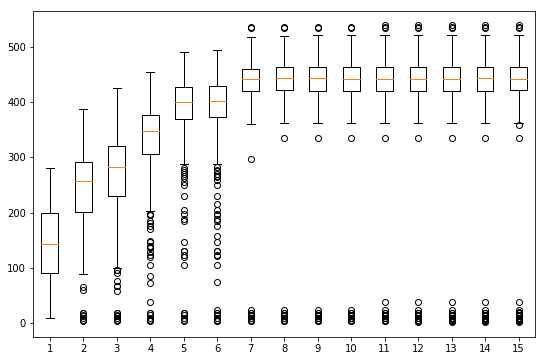
\includegraphics[scale = 0.35]{Figuresnew/boxplotpa.png}
    \caption{Number of infections over the $M$ samples (y-axis) vs $M/100$, i.e., the number of samples (in 100s) on the x-axis
for the Preferential Attachment (PA1) network.
}
    \label{fig:pa_boxplot}
\end{figure}


\begin{figure}[!h]
    \centering
    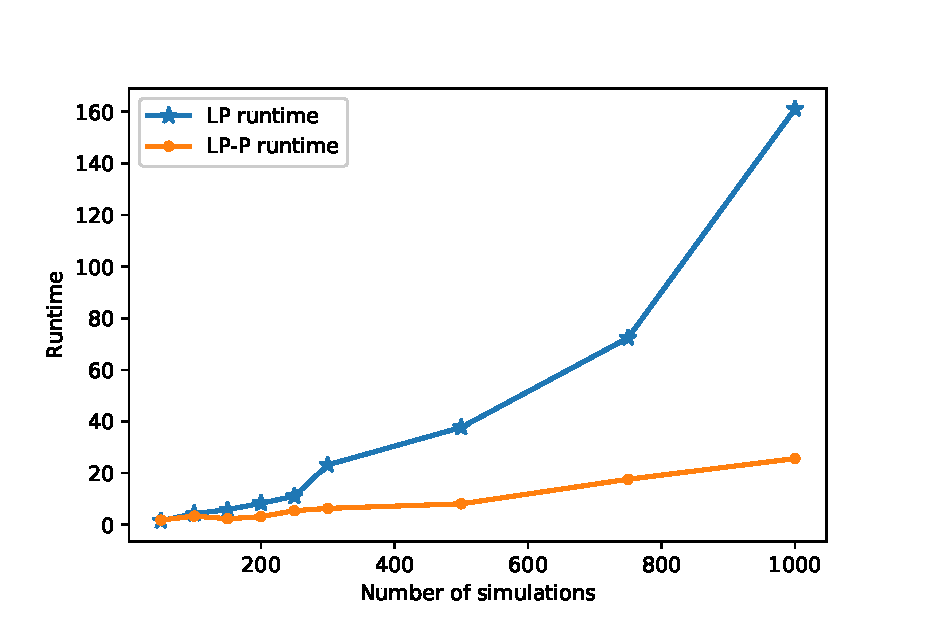
\includegraphics[scale = 0.5]{Figuresnew/pa1_runtime}
    \caption{Comparison of runtimes of Linear Programs with (LP-P) and without pruning (LP) on y-axis vs 
number of samples on x-axis for the PA1 network. }
    \label{fig:pa1pruningtime}
\end{figure}


\begin{figure}[!h]
    \centering
    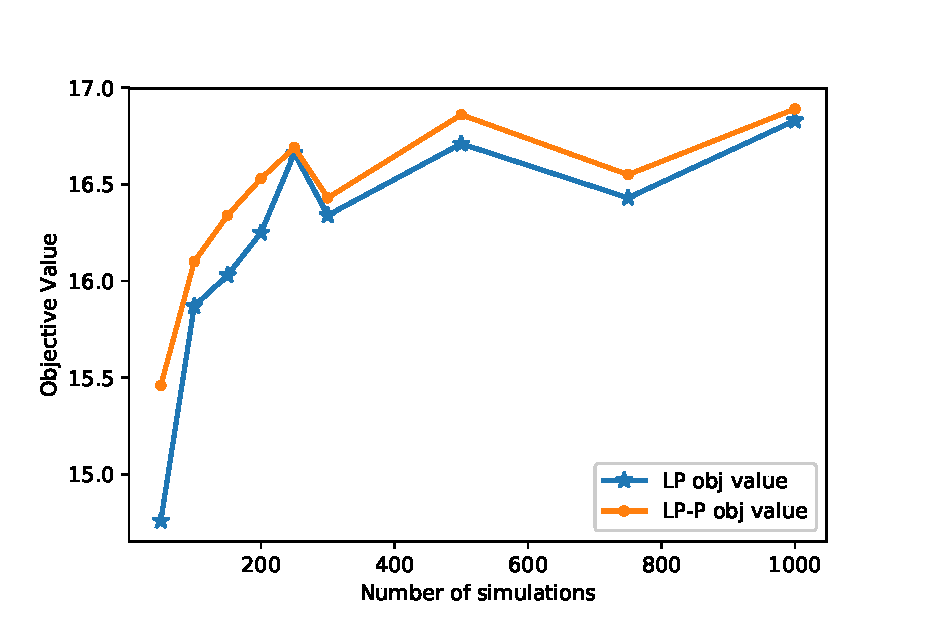
\includegraphics[scale = 0.5]{Figuresnew/pa1_objpruning}
    \caption{Comparison of the objective values of Linear Programs with (LP-P) and without pruning (LP) on the y-axis
vs the number of samples on the x-axis for the PA1 network. }
    \label{fig:pa1pruningobj}
\end{figure}

\begin{figure}[!h]
    \centering
    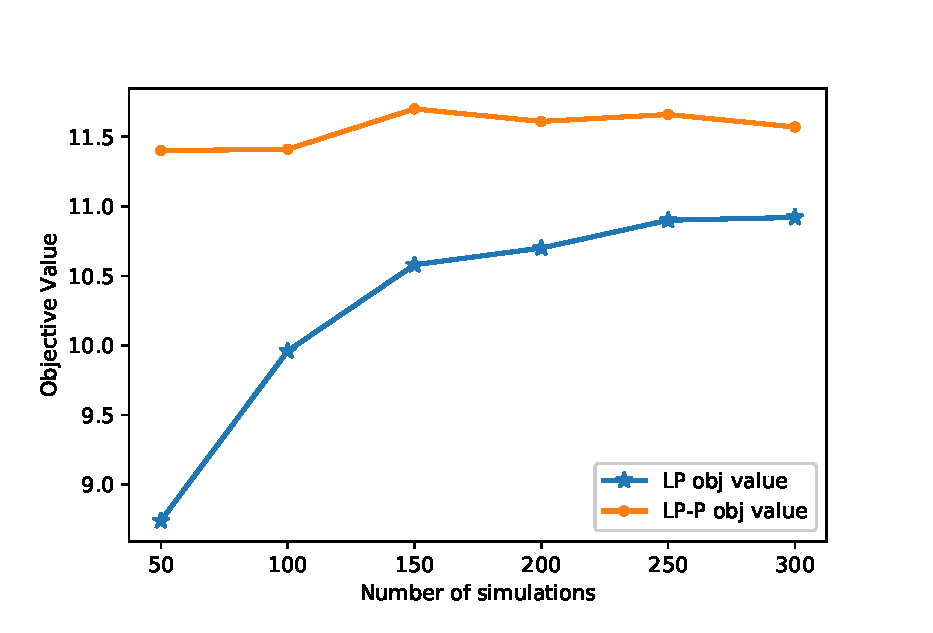
\includegraphics[scale = 0.5]{Figuresnew/portland_obj.eps}
    \caption{Comparison of objective values of Linear Programs with (LP-P) and without pruning (LP) on y-axis vs 
number of samples on x-axis for the Portland network. }
    \label{fig:portlandobj}
\end{figure}

\subsection{Performance Guarantees and comparison with baselines}

\subsubsection{Comparison to baselines}
Figures \ref{fig:performance} (a-d) show the objective value
for varying budgets for the \probone{} problem. We observe that \algo{} significantly outperforms
both the baselines. For social contact networks (Fig \ref{fig:performance}) (d), which are relatively dense,
the objective value from the eigenscore and degree baselines are over seven and three times that from
\algo{}, respectively, over the entire budget range. \algo{} outperforms eigenscore by a similar factor in Figure \ref{fig:performance} (c) as well.
Only in the smallest network (PA1), the differences between \algo{} and the baselines is not very high.
It is also surprising that the degree strategy is better than eigenscore in all the networks.

\subsubsection{Approximation Ratio}
We observe that the approximation ratio with respect to the objective value is close to 1. Figures \ref{fig:performance} shows that for all the four networks, the objective value of LP optimal solution almost coincides with that of \algo{}. Also, the approximation ratio with respect to budget violation is close to 1, in practice, shown in Figure \ref{fig:budgetviolation}.

%\begin{figure}[!h]
    %\centering
    %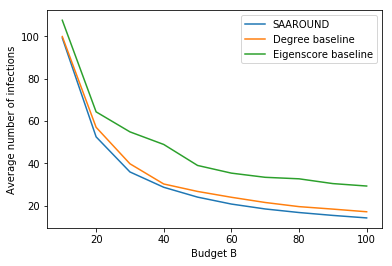
\includegraphics[scale = 0.55]{Figuresnew/pa1_approx}
    %\caption{Objective value (y-axis) vs budget (x-axis) for \algo{}, and the degree and eigenscore baselines for the PA1 network.}
%    \label{fig:pa1approx}
%\end{figure}
%
%\begin{figure}[!h]
  %  \centering
  %  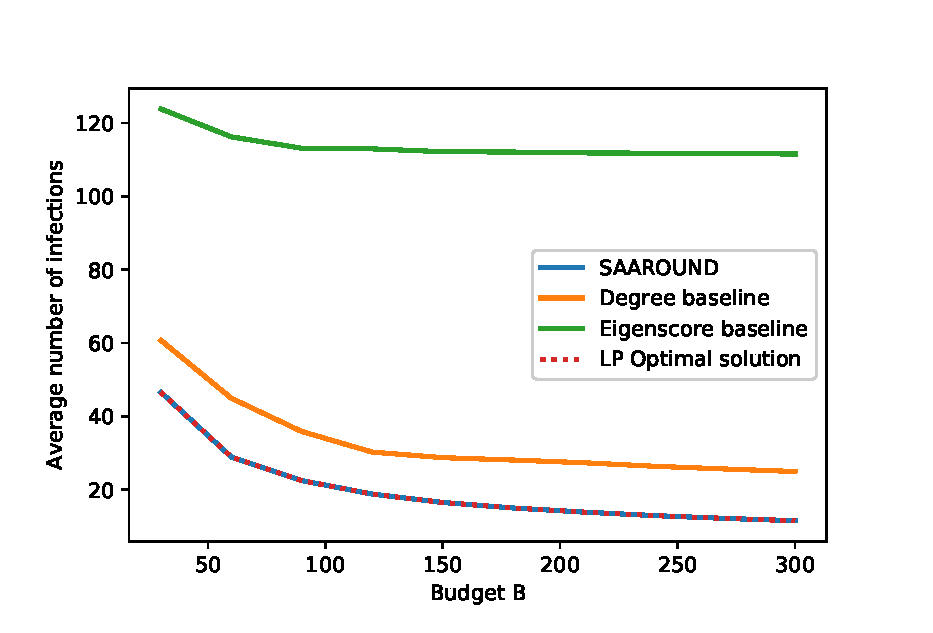
\includegraphics[scale = 0.55]{Figuresnew/barabasi_approx}
  %  \caption{Objective value (y-axis) vs budget (x-axis) for \algo{}, and the degree and eigenscore baselines for the PA2 network.}
  %  \label{fig:pa2approx}
%\end{figure}

%\begin{figure}[!h]
 %   \centering
 %   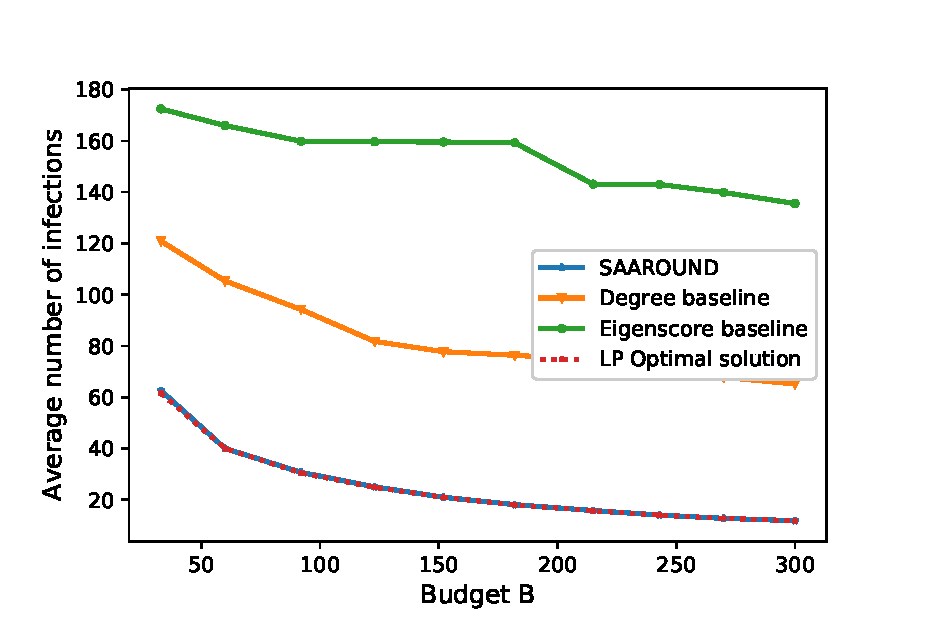
\includegraphics[scale = 0.6]{Figuresnew/mont_approx}
 %   \caption{Objective value (y-axis) vs budget (x-axis) for \algo{}, and the degree and eigenscore baselines for the Montgomery network.}
 %   \label{fig:mont-approx}
%\end{figure}

%\begin{figure}[!h]
    %\centering
    %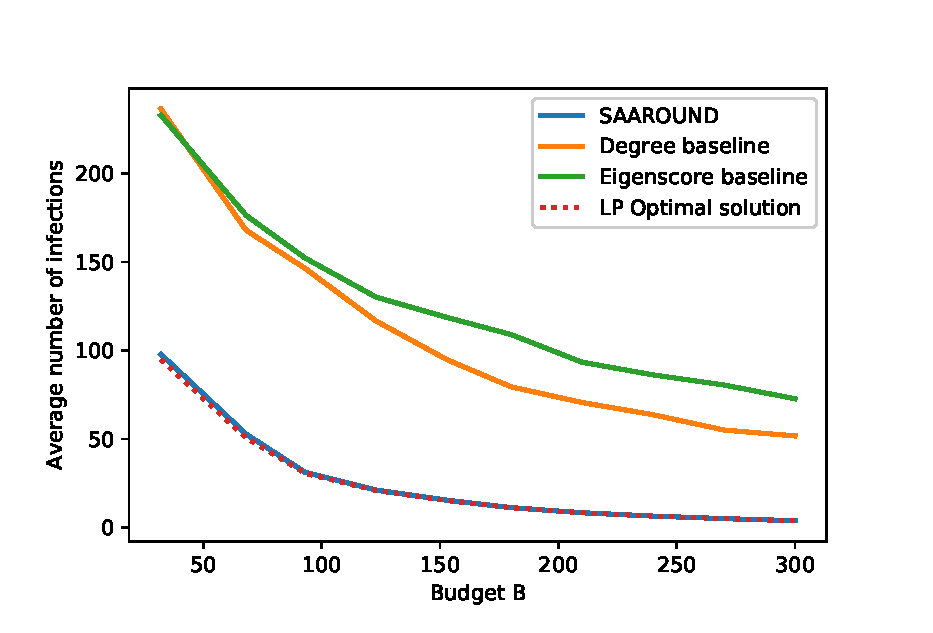
\includegraphics[scale = 0.6]{Figuresnew/smallworld_approx}
    %\caption{Objective value (y-axis) vs budget (x-axis) for \algo{}, and the degree and eigenscore baselines for the Small World network.}
%    \label{fig:mont-approx}
%\end{figure}

\begin{figure*}[ht] 
  \begin{minipage}[b]{0.5\linewidth}
    \centering
    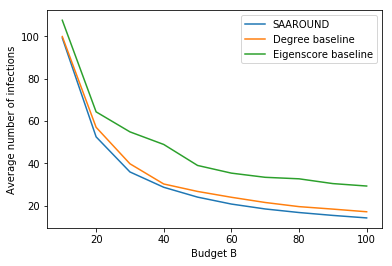
\includegraphics[scale=0.47]{Figuresnew/pa1_approx} 
    \caption*{a. Preferential1 (PA1)} 
    \vspace{1.1ex}
  \end{minipage}%%
  \begin{minipage}[b]{0.5\linewidth}
    \centering
    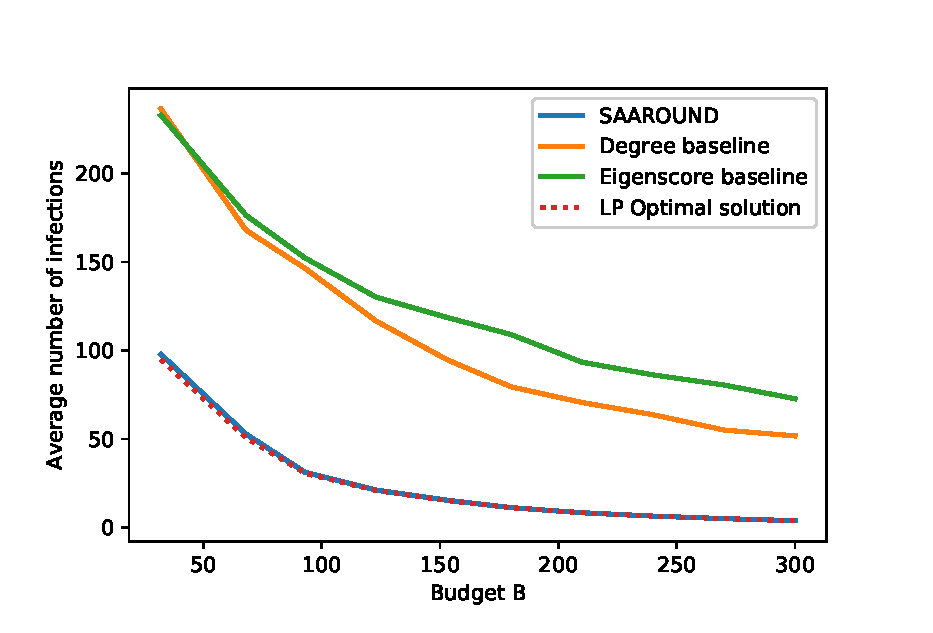
\includegraphics[scale=0.47]{Figuresnew/smallworld_approx} 
    \caption*{b. Small World (SW)} 
    \vspace{1.1ex}
  \end{minipage} 
  \begin{minipage}[b]{0.5\linewidth}
    \centering
    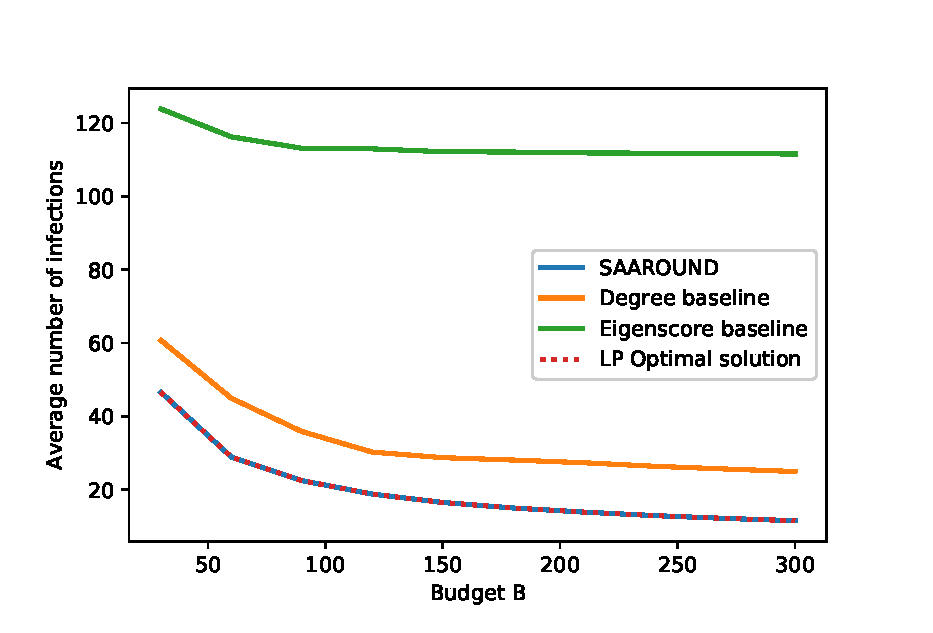
\includegraphics[scale=0.47]{Figuresnew/barabasi_approx} 
    \caption*{c. Preferential2 (PA2)} 
    \vspace{1.1ex}
  \end{minipage}%% 
  \begin{minipage}[b]{0.5\linewidth}
    \centering
    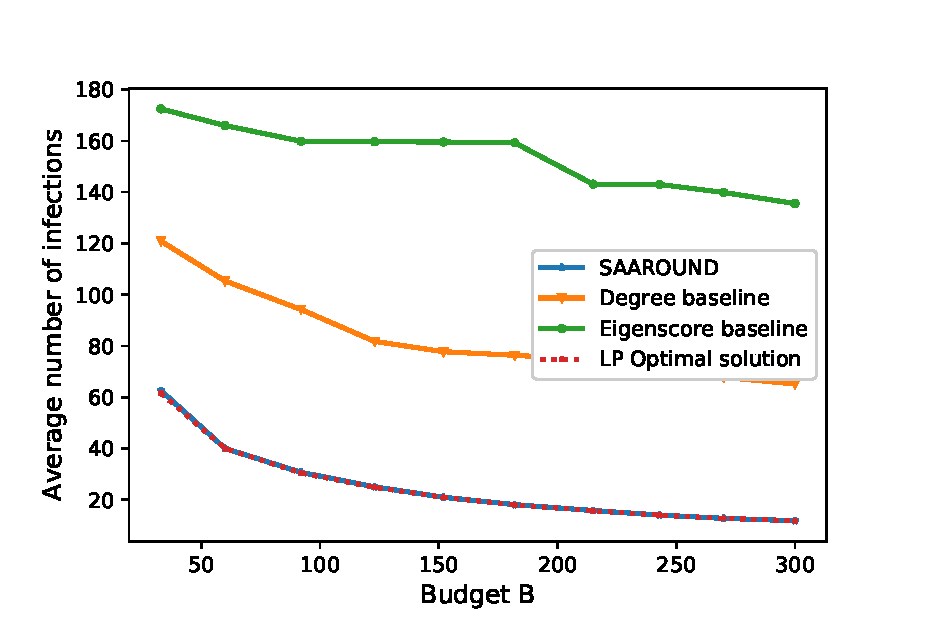
\includegraphics[scale=0.47]{Figuresnew/mont_approx} 
    \caption*{d. Montgomery} 
    \vspace{1.1ex}
  \end{minipage}
  \caption{Objective value (y-axis) vs budget (x-axis) for \algo{}, and the degree and eigenscore baselines for four networks.}
  \label{fig:performance} 
\end{figure*}

\begin{figure}[!h]
    \centering
    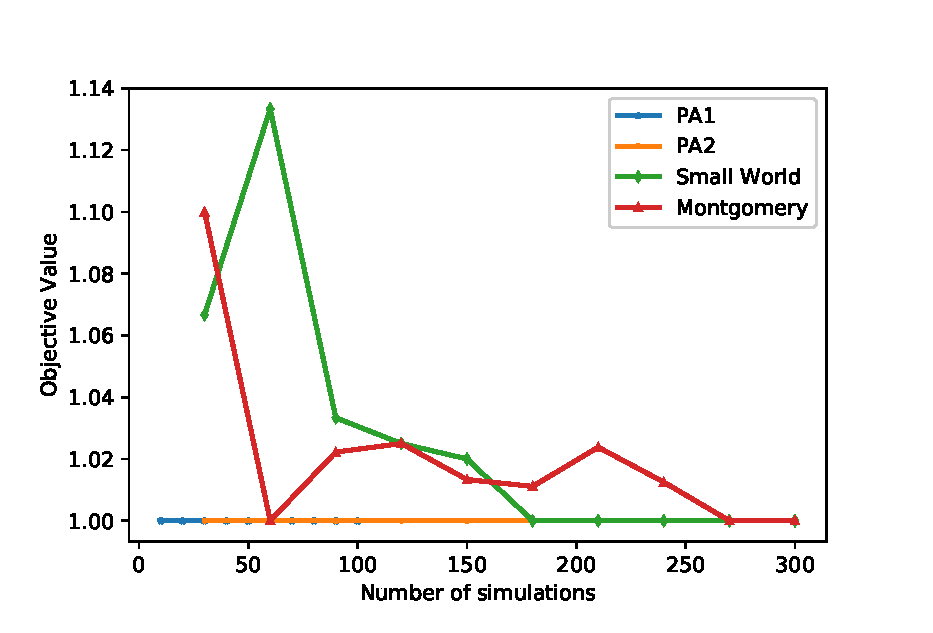
\includegraphics[scale = 0.45]{Figuresnew/budgetviolation}
    \caption{Budget approximation ratio: the ratio of interventions after rounding to the ones before rounding. X-axis is the original budget. Y-axis is the approximation ratio.}
    \label{fig:budgetviolation}
\end{figure}

\subsection{Two stage intervention and Structure of solution}
We study the \probtwo{}. In Figure \ref{fig:temporal}, we examine how the objective value $\expinf{}$ increases with $T$ in a two stage intervention, where $T$ is the time of the second stage, while the first intervention is performed at time step 0. We observe that $\expinf{}$ increases very rapidly with $T$.

Next, we examine the structure of the sets picked in each stage. Figure \ref{fig:montagedeg} shows a scatter plot of the node degree and age of the solution to \probtwo{} with $T=4$. We observe that there are slight differences between the sets $X_0$ and $X_4$: $X_0$ has slightly higher degree nodes, whereas $X_4$ has slightly lower age nodes. But more importantly, \emph{it is not the case that all high degree nodes are used in $X_0$}.
\begin{figure}[!h]
    \centering
    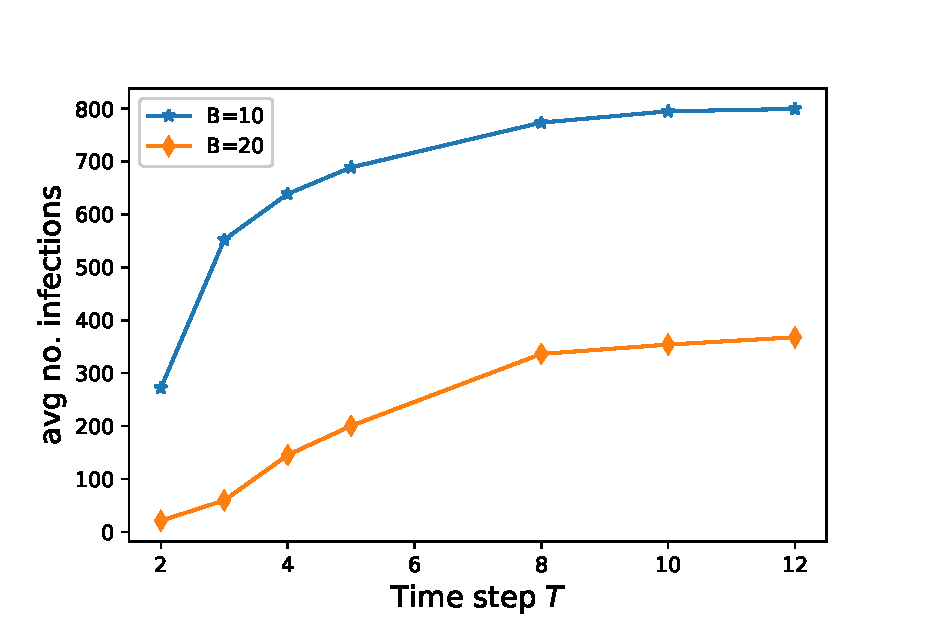
\includegraphics[scale = 0.45]{Figuresnew/twostage}
    \caption{CA-GrQc. Impact of varying $T$ in Two-stage Intervention. The X-axis corresponds to time step $T$ at which 2nd intervention is performed (1st intervention is at T =0). The Y-axis corresponds to the average number of infections over the simulations.}
    \label{fig:temporal}
\end{figure}

\begin{figure}[!h]
    \centering
    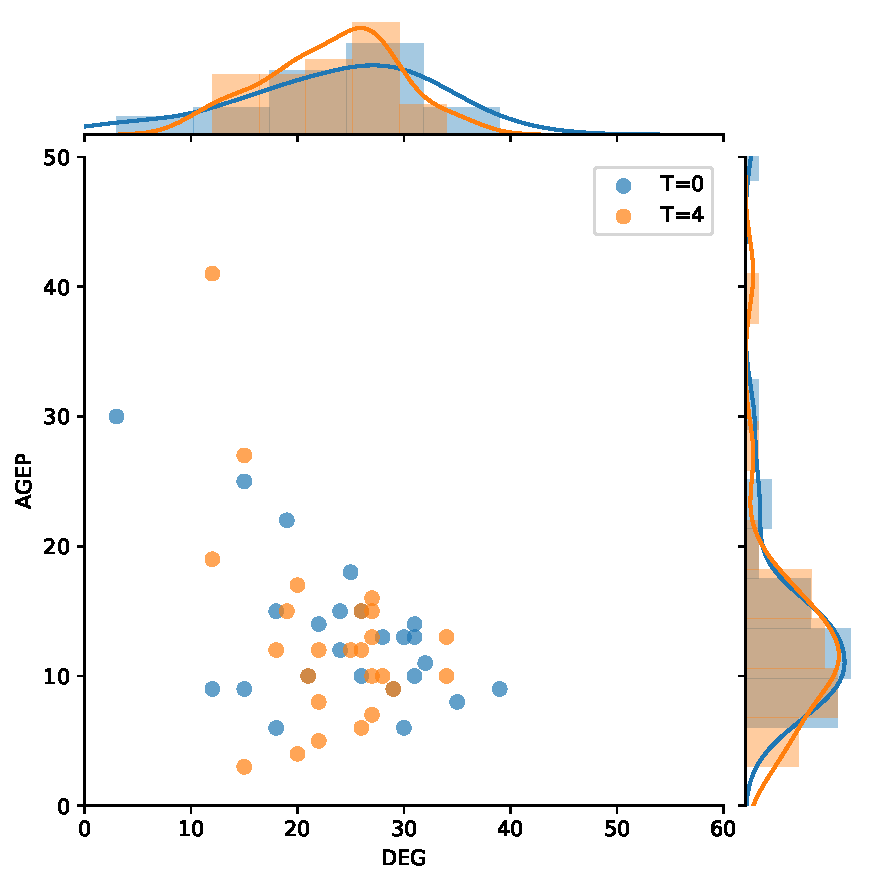
\includegraphics[scale = 0.5]{figures/t0_t4_compare_age_deg.pdf}
    \caption{Montgomery Graph: scatter plot of age and degree of nodes of the sets $X_0$ and $X_4$ in a solution to the 2-stage \prob{} with budgets $B_0 = B_4 = 25$.}
    \label{fig:montagedeg}
\end{figure}

\
%\subsection{Approximation Guarantees}


%\subsection{Characterizing Structure of Solution}


%\section{Experiments (OLD)}
\label{sec:experiments2}

We study the following questions. \\
\noindent
\textbf{1. Performance.} What is the approximation bound in practice, compared with the worst case guarantee given by Theorem \ref{theorem:algo}? How does the solution quality (in terms of the $\expinf{}$ objective) compare with other baselines, for the single stage version, i.e, $\mathcal{T}=\{0\}$?\\
\noindent
\textbf{2. Impact of time on the quality and structure of solution.} How does the objective value increase from a single stage to two stage? What kinds of nodes are picked in each stage?\\
\textbf{3. Interplay between information delay and intervention time.} Do we gain by waiting for information about the outbreak? By how much? At what point is it better not to wait?

% 1. What is the benefit of performing two stage non-adaptive interventions in comparison to the single stage strategies?

% 2. What is the impact of delay $\tau$ in the solutions to \probdelay for a fixed intervention time $T$ and budget $B$?

% 3. Given the delay in information $\tau$, how long can the policy makers wait for the information to perform the intervention? 

% 4. How does our algorithm perform on the montgomery network? What kind of people are picked for intervention for non-adaptive strategy with budget split? 

\subsection{Dataset and Methods}
We experiment with four very different kinds of networks, two random and two real, in order to fully explore the effect of network structure on the the results. We consider two random networks, namely the small world 
\cite{Kleinberg00thesmall-world}, and preferential attachment \cite{Barabasi509} models. We also study the results on the CA-GrQc collaboration network \cite{Leskovec:2007:GED:1217299.1217301}, since it is a type of social network. Finally, we consider a synthetic agent based population for Montgomery County, VA, constructed by a first principles approach by \cite{barrett:wsc09,eubank:nature04}. This has been used in several public health studies, e.g., \cite{singh:bmc19}. This network has a rich set of demographic attributes for each node, e.g., age, gender, and income.

\noindent
\textbf{Methods.}
We use \algo{} with one time step (i.e., $\mathcal{T}=\{0\}$, also referred to as single stage), or two time steps (i.e., $\mathcal{T}=\{0, T\}$, referred to as two stage, with $t=0$ being the first stage, and $t=T$ being the second stage). In the experiments involving delay, we use \algodelay{} with various $\tau$ and $T$ values. For the single stage problem, we use the strategy of picking nodes based on highest degree or eigenscore, which is the component in the first eigenvector of the graph's adjacency matrix \cite{tong:cikm12}.
There are no prior baselines for temporal vaccination. 



% The description  of datasets used in our experiments in presented in Table \ref{tab:datasets}. The Montgomery dataset is the social contact network of the population in the Montgomery County, VA. The nodes in this network corresponds to the people, while the edges correspond to the interaction of a pair of people that spans over 6 hours. CA-GrQc \cite{Leskovec:2007:GED:1217299.1217301} is a collaboration network, where the nodes correspond to the authors submitting papers to General Relativity and Quantum Cosmology category of Arxiv. An edge between two authors represents a collaboration between the authors. Both the Small World and the Preferential networks are random graphs generated using packages available in Networkx\cite{osti_960616}. The Small World is based on Kleinberg's small-world model \cite{Kleinberg00thesmall-world}, generated using ``navigable\_small\_world\_graph" function with the parameters $n = 50, p = 1, q = 5, r = 2, dim = 2$. Preferential is a random graph based on the preferential attachment model\cite{Barabasi509}, generated using ``barabasi\_albert\_graph'' function with the parameters $n=1000, m=2$.


\begin{table}[!h]
\centering
\begin{tabular}{llll}
\hline
 \textbf{Dataset} & \textbf{Nodes} & \textbf{Edges}   \\ \hline
 Montgomery & 70729 & 198138 \\
 CA-GrQc & 5242 & 14496\\
 Small World (SW) & 2500 & 14833 \\   
 Preferential (PA) & 1000 & 1996 \\ \hline
\end{tabular}
\caption{Description of datasets}
\label{tab:datasets}
\end{table}

\subsection{Performance}
We find that the approximation guarantee is a small constant in practice. This is shown in Figure \ref{fig:approx}, which compares the objective value of \algo{} with the fractional LP value, which is a lower bound on the optimum cost. In Figure \ref{fig:baseline}, we find that \algo{} gives a significant improvement over the baselines, in terms of the expected outbreak size.
\begin{figure}[!h]
    \centering
    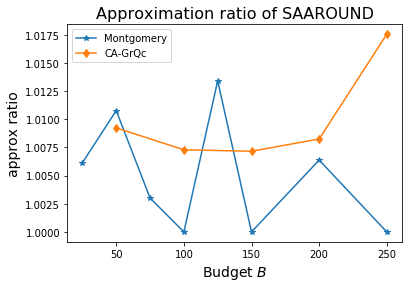
\includegraphics[scale = 0.35]{figures/approx.png}
    \caption{Approximation Ratio of \algo{} on real datasets.}
    \label{fig:approx}
\end{figure}
 

\begin{figure}[!h]
    \centering
    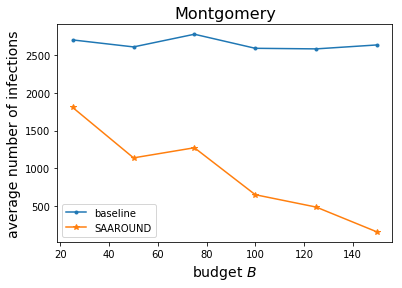
\includegraphics[scale = 0.5]{figures/baslinecomp.png}
    \caption{Montgomery. Comparison of \algo{} performance with degree based greedy algorithm as baseline. X-axis corresponds to the budget $B$ on the interventions, while the Y-axis corresponds to the average number of infections over all simulations. 
    }
    \label{fig:baseline}
\end{figure}
 
 
\subsection{Two stage interventions}
We study the two stage version of \prob{}. Here no information about the outbreak is available, and so, clearly, earlier is better, i.e., if the entire budget is available at time $0$, it is better to use it right away. In Figure \ref{fig:temporal}, we examine how the objective value $\expinf{}$ increases with $T$ in a two stage intervention, where $T$ is the time of the second stage. We observe that $\expinf{}$ increases very rapidly with $T$.

Next, we examine the structure of the sets picked in each stage. Figure \ref{fig:montagedeg} shows a scatter plot of the node degree and age of the solution to a two stage version with $T=4$. We observe that there are slight differences between the sets $X_0$ and $X_4$: $X_0$ has slightly higher degree nodes, whereas $X_4$ has slightly lower age nodes. But more importantly, \emph{it is not the case that all high degree nodes are used in $X_0$}.

% We call the intervention strategy without any information on the epidemic state as non-adaptive interventions. In such strategies, we can do at all interventions at a particular time step $T$ or do it at multiple time steps with the budget split over these times. In our experiments, we present the latter case for performing interventions at two time steps: (i) one set of interventions at $T = 0$ with $B/2$ budget and (ii) another set of interventions at $T = t$ with the remaining budget.
\begin{figure}[!h]
    \centering
    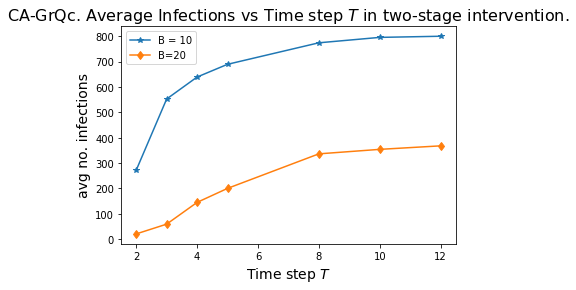
\includegraphics[scale = 0.4]{figures/twostage.png}
    \caption{CA-GrQc. Impact of varying $T$ in Two-stage Intervention. The X-axis corresponds to time step $T$ at which 2nd intervention is performed (1st intervention is at T =0). The Y-axis corresponds to the average number of infections over the simulations.}
    \label{fig:temporal}
\end{figure}

\begin{figure}[!h]
    \centering
    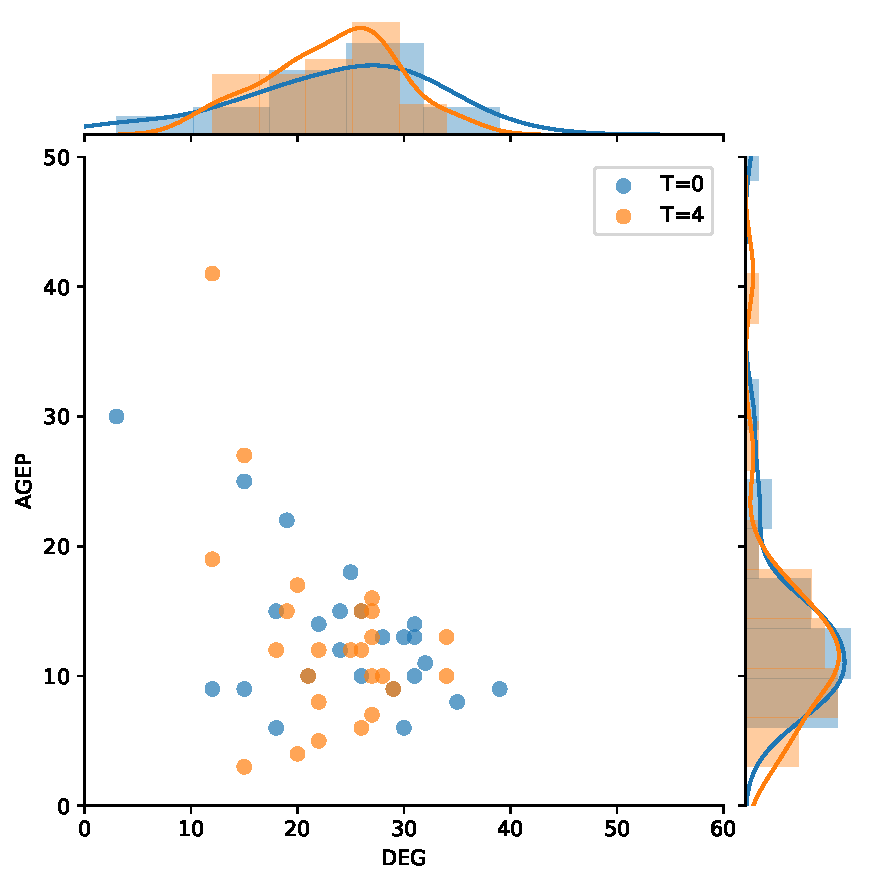
\includegraphics[scale = 0.45]{figures/t0_t4_compare_age_deg.pdf}
    \caption{Montgomery Graph: scatter plot of age and degree of nodes of the sets $X_0$ and $X_4$ in a solution to the 2-stage \prob{} with budgets $B_1 = B_4 = 25$.}
    \label{fig:montagedeg}
\end{figure}

\subsection{Interplay between information delay and intervention time}

Here, we consider the \probdelay{} problem, and study the interplay between the information delay $\tau$ and the time $T$ at which the intervention is done. 

\begin{figure}[!h]
    \centering
    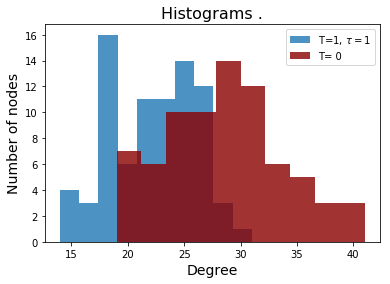
\includegraphics[scale = 0.6]{figures/histogram.png}
    \caption{X-axis corresponds to degree of nodes picked for intervention at $T=0$. Y-axis corresponds to number of nodes. The histogram in blue corresponds to node picked for intervention at $T = 1$ with $\tau = 1$. The histogram in dark red corresponds to the picked for intervention at $T = 0$.}
    \label{fig:hist}
\end{figure}


\subsubsection{Impact of delay in information}
\begin{figure}[!h]
    \centering
    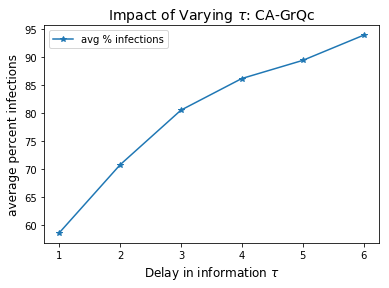
\includegraphics[scale = 0.5]{figures/varytauGrQc.png}
    \caption{Impact of varying $\tau$ for fixed T = 7 and B = 50: CA-GrQc}
    \label{fig:T7tau}
\end{figure}

We study the impact of delay of information $\tau$ for a fixed budget $B$ and time of intervention $T$. Figure \ref{fig:T7tau} shows that the average \% infected increases with the increase in $\tau$ value, for a fixed $T = 7$ and budget $B=50$. The average percentage infections is the average of the percentage of infections over the simulations.


%We observe that as the delay $\tau$ increases, the number of infections increases rapidly. Figure \ref{fig:T7tau} shows this phenomenon on CA-GrQC network for a fixed time of intervention $T = 7$ and budge $B = 50$. The average percentage infections is the average of the percentage of infections over all the epidemic simulations. 


\subsubsection{How long to wait for information}
We use \algodelay{} to examine when it is beneficial to wait for information before intervention, when is it not, by varying $\tau, T, B$ in Figure \ref{fig:howlong} for the Montgomery county, PA and SW networks, respectively. In each figure,
the red dashed line corresponds to the expected number of infections, i.e., the $\expinf(\cdot)$ objective, if the intervention is performed at time $0$. Each curve corresponds to a different $\tau$ value, and shows the $\expinf(X_T)$ objective on the $y$-axis, and the time $T$ on the $x$-axis. As long as the curves are below the red dashed line, an intervention at that time, taking the delayed information into account, is better than doing it at time $0$.

The time at which the curves intersect the red dashed line varies by network. For the Montgomery county network, $T$ is close to 14. But it is much smaller for both the PA and SW networks, and for them it does not help to delay the intervention much. Interestingly, for the Montgomery county network, we find the time at which the intersection happens is actually past the peak, shown in Figure \ref{fig:howlong}. We present the average epicurve of Montgomery dataset in Figure \ref{fig:epicurve}.


% In this section, we discuss when is it beneficial to wait for information before intervention, when is it not. We present results on the Small World, Preferential, and the Montgomery datasets. We fix the budget to $B$ and run our algorithm for various choices of intervention time $T$ and $\tau$. In case of the Small World dataset, we observe that waiting for information beyond $T= 2$ when $\tau = 1$ is worse than performing interventions at the beginning. When $\tau = 3$, it is always better to perform interventions at the beginning. This can be seen in Figure \ref{fig:swdelay}, where the red dashed line, corresponding to the number of infections after performing intervention at $T = 0$ cuts the curve corresponding to $\tau = 1$ before $T = 3$.

% The average epicurve corresponding to the average number of infections at each time step over all simulations is presented in Figure \ref{fig:epicurve}. The peak is around time step $T = 4$. As shown in Figure \ref{fig:montgodelay}, it is beneficial to wait for information when the delay is small (i.e. $\tau \in \{2, 4\}$). Our experiments suggest that, in such population, it is beneficial to wait for information at least till before peak.

\begin{figure}[!h]
    \centering
    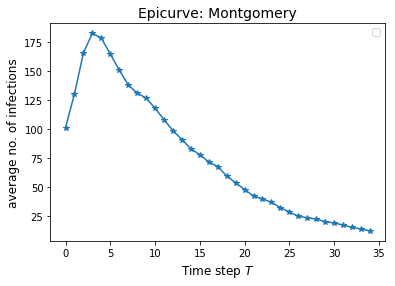
\includegraphics[scale = 0.5]{figures/epicurve.png}
    \caption{Epicurve for Montgomery: average number of infections at each time step $T$.}
    \label{fig:epicurve}
\end{figure}

\begin{figure*}[!h]

\centering
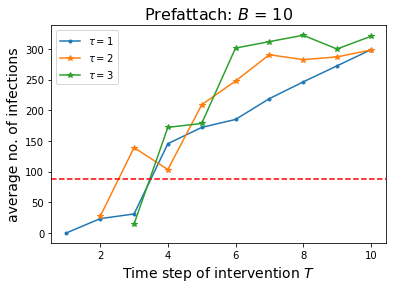
\includegraphics[width=.37\textwidth]{figures/prefattach_howlong.png}\hfill
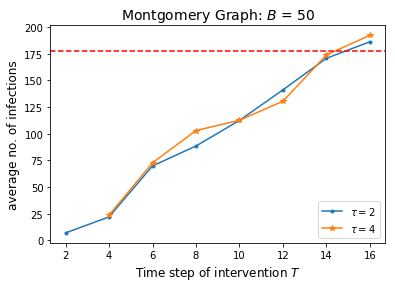
\includegraphics[width=.37\textwidth]{figures/montgo_howlong.png}\hfill
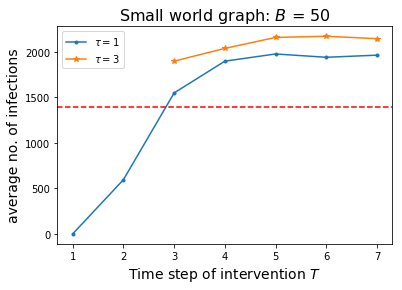
\includegraphics[width=.37\textwidth]{figures/sw_howlong.png}

\caption{How long to wait for information? In each plot, X-axis corresponds to the time of intervention. Budget $B = 10$. Y-axis corresponds to the average number of infections. The dashed horizontal red line corresponds to the number of infections if the intervention is performed at the beginning of the epidemic.}
\label{fig:howlong}

\end{figure*}




\section{Related work}
\label{sec:related}

\subsection{Public health policy planning and use of diffusion models}
Public health policy analysis relies heavily on mathematical models of SIR type processes, e.g., \cite{lofgren:pnas14,anderson+m:book}. As discussed earlier, there are two broad classes of models. The first involves using a system of coupled differential equations to represent the dynamics, e.g., \cite{medlock:science09,AAAI1816714,venkataramanan:ichi17}. These do not have any closed form solutions, in general, and when the system is not very large, it can be solved by brute force local search methods \cite{medlock:science09}. For some types of models, greedy strategies have been used \cite{AAAI1816714,venkataramanan:ichi17}. 
The second is network based, and uses a stochastic diffusion model for the spread of the disease \cite{marathe:cacm13,halloran:pnas08,lofgren:pnas14,eubank:nature04,gk06}. Such models have been found to be more powerful and useful for epidemic spread on large heterogeneous populations, where the complete mixing assumptions of differential equation models are not valid.

During any large outbreak, public health agencies solve a variety of models, and make plans and guidelines based on the results,
e.g., during the 2009 swine flu \cite{medlock:science09}, and
the 2014 Ebola outbreak \cite{lofgren:pnas14}. Such studies typically explore the space of different possible interventions, within given resource constraints. Therefore, there is a lot of interest in the design of optimal or near-optimal interventions.

\subsection{Resource optimization to control epidemic spread}
There is a lot of work on this topic, and we summarize the main research directions relevant to \prob{}.

\noindent
\textbf{Firefighter problems}, e.g., \cite{anshelevich09,Finbow2009TheFP,Chalermsook:2010:RMF:1873601.1873709}. 
This is most closely related to \prob{}. The basic version of the problem is to
determine a temporal intervention $\X=\{X_t: t=1,\ldots,n\}$, such that $|\X_t|\leq B$,
and the number of nodes not infected (i.e., saved) is maximized (this is referred to as the Max-Save version).
The disease model is a SI process with $p=1$ (so this is a deterministic model).
The Max-Save version cannot be approximated within an $\Omega(n^{\epsilon})$ factor for any $\epsilon < 1$, in general graphs.
A related problem is the Min-Budget version, for which an $O(\sqrt{n})$ approximation is 
possible \cite{Chalermsook:2010:RMF:1873601.1873709}.
This work corresponds to \emph{non-spreading} interventions. Better approximations are possible for the setting in which
the vaccination is also a \emph{spreading} process.
We refer to Finbow et al. \cite{Finbow2009TheFP} for an extensive survey on the firefighter problems.
One of the few works on the firefighter problem with a stochastic disease model (i.e., $p<1$) is by
Tennenholtz et al. \cite{DBLP:journals/corr/abs-1711-08237}, who formalize the problem as a Markov Decision Process (MDP),
and compute an optimal solution for trees.  One of the main differences between this and our paper is that
the MDP formulation of \cite{DBLP:journals/corr/abs-1711-08237} makes the problem \emph{adaptive},
i.e., it is possible to use information about which nodes are infected before time $t$, in designing 
the intervention $\X_t$. In contrast, \prob{} only considers a non-adaptive setting, and the intervention
has to be determined ahead of time.

\noindent
\textbf{Optimization of spectral properties.}
A key result in epidemic modeling is a characterization of an outbreak in terms of spectral properties,
namely the first eigenvalue (also referred to as the spectral radius, and denoted by $\lambda_1$)

\cite{PreciadoVM13_2,PreciadoVM13,PreciadoVM14,SahaSDM15,Ogura2017}. Much of this work is based on
controlling spectral properties, but does not give any guaranteed bounds on the expected outbreak size;
(2) Firefighter problem, which can be viewed as \prob{} on SI model with with $p=1$, e.g.,
\cite{anshelevich09,Finbow2009TheFP}. Rigorous bounds are known for the number infected and saved.
However, this has not been studied much for the case where $p<1$, except \cite{DBLP:journals/corr/abs-1711-08237},
which only gives rigorous algorithms for trees.
A special case of this problem is with work of \cite{Aspnes:2005}, which considers \prob{} but with
the intervention specified at time 0;
(3) Static interventions in SIR models, e.g., \cite{zhang2015controlling,YaoSDM2014}, which also do not
directly bound the expected outbreak size,
(4) Heuristics for picking nodes based on degree or centrality, e.g., \cite{PhysRevLett.91.247901,Miller2007EffectiveVS},
which work for all models but give no guarantees.
In summary, none of the prior results give rigorous results for \prob{}, to minimize the expected
number of infections, with budget constraints over time, in SIR models of epidemics, with transmission probability less than $1$.


There has been a lot of work on optimizing vaccine allocation. A lot of it has been based on the idea of picking nodes to vaccinate, based on their eigenscore, i.e., their component values in the first eigenvector \cite{PreciadoVM13_2,PreciadoVM13,PreciadoVM14,SahaSDM15,Ogura2017,zhang2015controlling,YaoSDM2014}. It is not clear how to incorporate temporal constraints and delay and information within such formulations. In particular, these results do not incorporate the effects of where the sources are, and instead try to shift the phase transition for a large outbreak, which is in terms of the spectral radius. As we have discussed, such static interventions don't do very well.



\section{Conclusions}
\label{sec:conc}

We develop the first rigorous algorithm for temporal intervention design to control the spread of epidemics on networks. Our algorithm performs significantly better than standard baselines, and has near-optimal approximation guarantee in practice. Our main techniques are linear programming based rounding and the sample average approximation technique.
We find that the temporal dimension leads to significant changes in the solution quality and structure. Finally, we study the impact of delay and intervention time. We find that in some networks, there is a point up to which waiting helps. Our methods can help in public health policy planning and response to large outbreaks. 


\clearpage
{\small
\bibliographystyle{ACM-Reference-Format}
\bibliography{references}
}

\clearpage
\section{Appendix}
\label{appendix}

\subsection{Choosing model parameters}


\begin{figure}[!h]
    \centering
    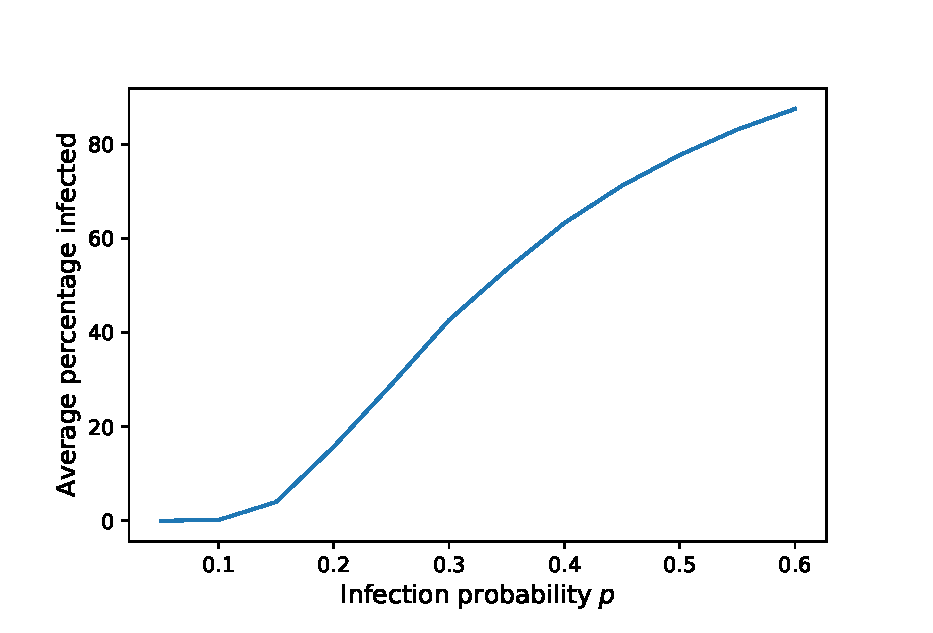
\includegraphics[scale = 0.55]{Figuresnew/PA_attackrates.eps}
    \caption{Preferential: p vs avg. percent infected.)}
    \label{fig:PA_ar}
\end{figure}

\begin{figure}[!h]
    \centering
    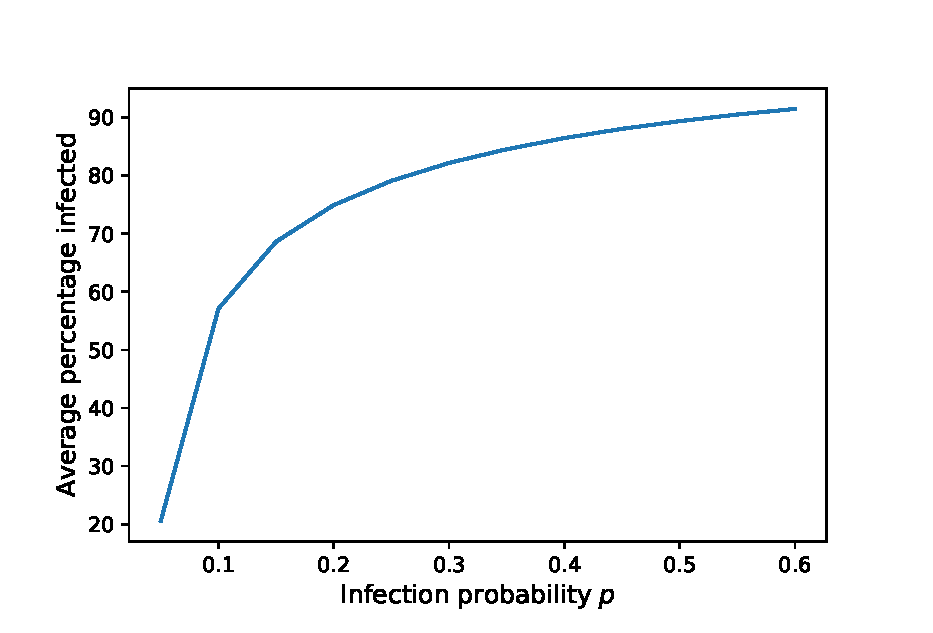
\includegraphics[scale = 0.55]{Figuresnew/montgo_attackrates.eps}
    \caption{Montgomery: p vs avg. percent infected.}
    \label{fig:montgo_ar}
\end{figure}



\begin{figure}[!h]
    \centering
    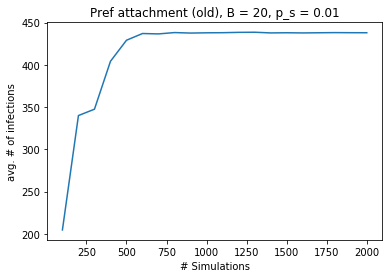
\includegraphics[scale = 0.6]{Figuresnew/simulations.png}
    \caption{Simulation vs average infected (Preferential Attachment)}
    \label{fig:pa_simvsavg}
\end{figure}


\end{document}
